\chapter{Frequency response of RME FIREFACE UCX}\label{Frequency_response_of_RME_FIREFACE_UCX}
A measurement was conducted to assess the frequency response of the RME FIREFACE UCX. Because all the measurements in this project involve the FIREFACE ucx, the frequency response is of interest. To measure the frequency response, the function from \autoref{appendix:transfer_function} is used.

\section*{Materials and setup}
The following materials are used:
\begin{itemize}
\item RME FIREFACE ucx (Soundcard)
\begin{itemize}[noitemsep]
\item AAU-number: 108230
\item Serial number: 23811948
\end{itemize}
\item MATLAB 2017b (PC - Software)
\item IRmeas_fft (software) \autoref{appendix:transfer_function}
\item jack to jack cable
\end{itemize}

\begin{figure}[H]
\centering
\begin{picture}(0,0)%
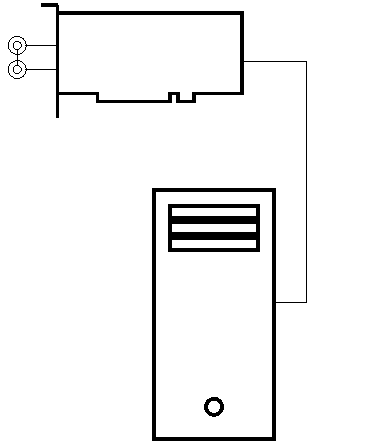
\includegraphics{rme_transfer_function.pdf}%
\end{picture}%
\setlength{\unitlength}{2818sp}%
%
\begingroup\makeatletter\ifx\SetFigFont\undefined%
\gdef\SetFigFont#1#2#3#4#5{%
  \reset@font\fontsize{#1}{#2pt}%
  \fontfamily{#3}\fontseries{#4}\fontshape{#5}%
  \selectfont}%
\fi\endgroup%
\begin{picture}(4090,4926)(8176,-7474)
\put(8191,-3661){Out}%
\put(9271,-3211){Sound Card}%
\put(9971,-6361){Computer}%
\put(11836,-4696){USB}%
\put(8281,-2806){In}%
\end{picture}%
\caption{Setup for measuring transfer function}
		\label{fig:appendix:rme_response}
\end{figure}

\section*{Test procedure}


\begin{enumerate}
\item The devices are set up as in \autoref{fig:appendix:rme_response}.
\item The sample rate is set to \SI{44.1}{\kilo\hertz}
\item The cable is connected between input 1 and output 1
\item The input gain at input 1 is set to \SI{20}{\decibel}
\item The output \texttt{playgain} is set to \SI{-18}{\decibel}
\item The input and output channel is specified in the MATLAB function "SynchronizedPlaybackAcquirer" 
\item IRmeas_fft (software) \autoref{appendix:transfer_function} is preformed
\item The transfer function is plotted from \SI{20}{\hertz} to \SI{20}{\kilo\hertz}
\end{enumerate}

\section*{Results}



\autoref{fig:appendix:rme_response_result} illustrates, that the soundcard only diverges \SI{0.26}{\decibel} from a linear frequency response at a frequency range from \SI{20}{\hertz} to \SI{20}{\kilo\hertz} between the output and input signal. 

\begin{figure}[H]
	\centering
	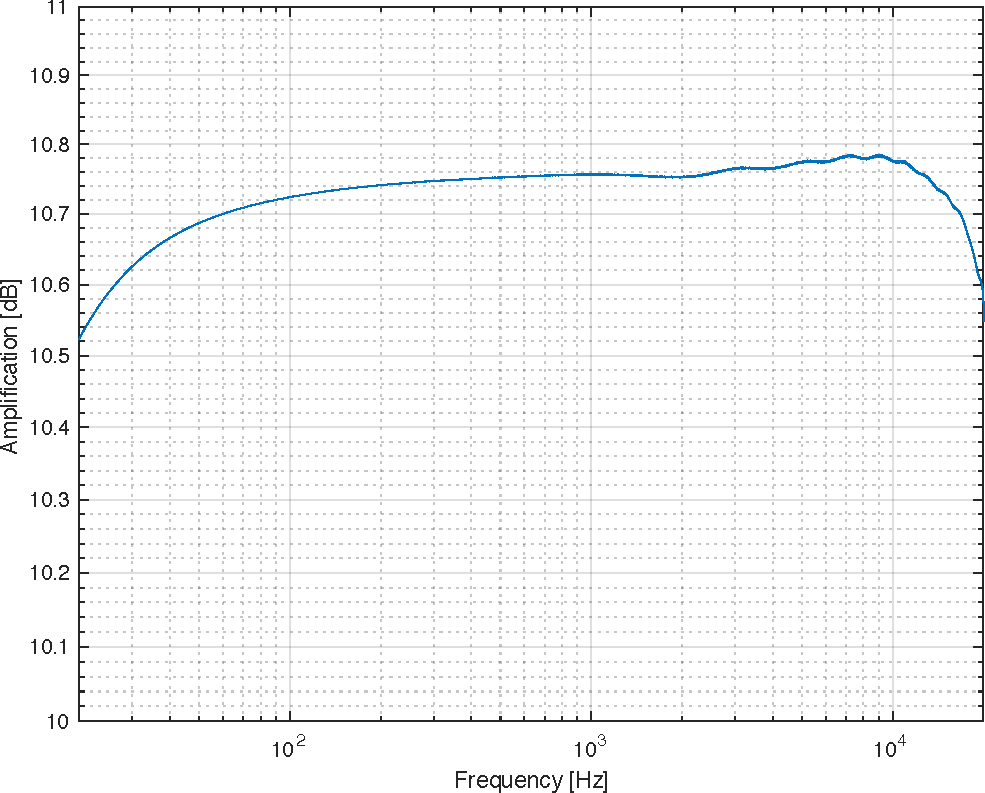
\includegraphics[width=1\textwidth]{RME_FIREFACE_UCX_tf.pdf}
	\caption{The frequency response of the RME FIREFACE UCX with input sensitivity at 20}
		\label{fig:appendix:rme_response_result}
\end{figure}

\section*{Conclusion}
It can be concluded that en RME_FIREFACE_UCX have a non linearity of \SI{0.26}{\decibel} when the input gain is at \SI{20}{\decibel} and the output \texttt{playgain} is at \SI{-18}{\decibel}


